\documentclass[spanish, fleqn]{article}
\usepackage{babel}
\usepackage[utf8]{inputenc}
\usepackage{amsmath,amsfonts}
\usepackage{enumitem}
\usepackage[colorlinks, urlcolor=blue]{hyperref}
\usepackage{fourier}
\usepackage{tikz}
\usetikzlibrary{shapes.geometric}
\usetikzlibrary{positioning}
\usepackage{verbatim}
\usepackage[top = 2.5cm, bottom = 2cm, left = 2.5cm, right = 2.5cm]{geometry}
\usepackage{parskip}
\setlength{\parskip}{2mm}
\newcommand{\num}{3}

\title{Estructuras Discretas \\
	Tarea \#\num \\
	``TLUITO GAIENL''}
\author{Andrés Navarro\\(201673001-K)}

\begin{document}
	\maketitle
	\thispagestyle{empty}
	
	% Pregunta 1
	\section*{Pregunta 1}
	
	Se tiene un pentágono regular y 3 colores diferentes para colorear su vértices. Calcule el número de maneras de colorear el péntagono, considerando que no es necesario usar todos los colores para cada coloreo y que se consideran equivalentes dos maneras de colorear si resultan iguales al rotar el pentágono.
	
	\begin{center}	
		\begin{minipage}{.22\textwidth}
			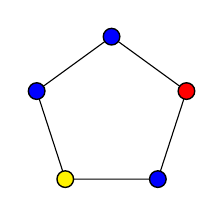
\begin{tikzpicture}
				\draw (90:1cm) -- (18:1cm) -- (306:1cm) -- (234:1cm) -- (162:1cm) -- (90:1cm);
				\draw[line width=.5pt,fill=blue] (90:1cm) circle (3pt);
				\draw[line width=.5pt,fill=red] (18:1cm) circle (3pt);
				\draw[line width=.5pt,fill=blue] (306:1cm) circle (3pt);
				\draw[line width=.5pt,fill=yellow] (234:1cm) circle (3pt);
				\draw[line width=.5pt,fill=blue] (162:1cm) circle (3pt);
			\end{tikzpicture}
		\end{minipage}	
		\begin{minipage}{.14\textwidth}
			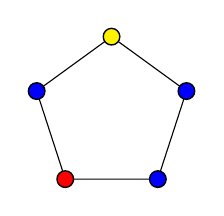
\begin{tikzpicture}
				\draw (90:1cm) -- (18:1cm) -- (306:1cm) -- (234:1cm) -- (162:1cm) -- (90:1cm);
				\draw[line width=.5pt,fill=yellow] (90:1cm) circle (3pt);
				\draw[line width=.5pt,fill=blue] (18:1cm) circle (3pt);
				\draw[line width=.5pt,fill=blue] (306:1cm) circle (3pt);
				\draw[line width=.5pt,fill=red] (234:1cm) circle (3pt);
				\draw[line width=.5pt,fill=blue] (162:1cm) circle (3pt);
			\end{tikzpicture}
		\end{minipage}
	\end{center}
	\begin{center}
		Figura 1: ejemplo de 2 maneras de colorear equivalentes
	\end{center}

	En un principio tenemos una secuencia con repeticiones, dado que cada vértice del pentágono puede tomar cualquiera de los 3 colores:
	\begin{align*}
	\text{Casos posibles}=3\cdot 3\cdot 3\cdot 3\cdot 3=243
	\end{align*}	
	
	Ahora bien, según el enunciado, se deben tomar como equivalentes 2 casos que al rotarse de cierta manera sean el mismo, por lo que tenemos que cada caso debería tener 4 casos equivalentes (5 representan 1). Sin embargo, tenemos 3 casos únicos que no se presentan como 5 en el conteo de casos posibles anterior, que corresponden a los que en cada punto del pentágono se tiene el mismo color.
	
	Por lo que tenemos los siguiente:	
	\begin{align*}
	&\text{Casos posibles que se repiten 5 veces}=3\cdot 3\cdot 3\cdot 3\cdot 3-3=240\\
	&\text{Dividimos por 5 para eliminar las maneras de colorear equivalentes}\\
	&\text{Casos posibles}=240/5=48
	\end{align*}
	
	Con esto obtenemos las maneras de colorear sin que estas se repitan 5 veces, pero a esto les debemos sumar los 3 casos que no se repetían 5 veces.
	
	Finalmente tenemos:
	\begin{align*}
	\text{Maneras de colorear}=48+3=51
	\end{align*}		
	
	\section*{Pregunta 2}
	Considere la palabra \texttt{EFERVESCENTEMENTE}:
    \begin{enumerate}
    \item ¿De cuántas maneras se pueden ordenar las letras de \texttt{EFERVESCENTE}?
    
    Dado que la palabra es formada por 12 letras, y 5 de ellas son ``E'', tenemos:
    \begin{align*}
    \text{Maneras de ordenar}=\frac{12!}{5!}= 3991680
    \end{align*}
    \item ¿De cuántas maneras se pueden ordenar las letras de \texttt{ME\textsubscript{1}NTE\textsubscript{2}}?
    
    Dado que la palabra es formada por 5 letras, haciendo distinción en las 2 ``E'', tenemos:
    \begin{align*}
    \text{Maneras de ordenar}=5!= 120
    \end{align*}
    \item Mapee los ordenamientos de \texttt{ME\textsubscript{1}NTE\textsubscript{2}} a \texttt{MENTE}, ¿qué clase de mapa es este?
    
    \texttt{ME\textsubscript{1}NTE\textsubscript{2}} $\rightarrow$ \texttt{MENTE}    
   
    \vspace{-0.2cm}\texttt{ME\textsubscript{2}NTE\textsubscript{1}} 
    
    Corresponde a un mapa 2 a 1.
    \item ¿Qué clase de mapa es el que lleva de \texttt{E\textsubscript{1}FE\textsubscript{2}RVE\textsubscript{3}SCE\textsubscript{4}NTE\textsubscript{5}ME\textsubscript{6}NTE\textsubscript{7}} a  \texttt{EFERVESCENTEMENTE}?
    
    Es un mapa 7! a 1, ya que las todas las ``E'' con subíndice pasan a ser solo ``E''.
    
    \item ¿Cuántos ordenamientos de \texttt{E\textsubscript{1}FE\textsubscript{2}RVE\textsubscript{3}SCE\textsubscript{4}N\textsubscript{1}T\textsubscript{1}E\textsubscript{5}ME\textsubscript{6}N\textsubscript{2}T\textsubscript{2}E\textsubscript{7}} hay?
    
    Dado que la palabra es formada por 17 letras haciendo distinción en todas las letras que se repiten, tenemos:
    \begin{align*}
    \text{Maneras de ordenar}=17!= 355687428096000
    \end{align*}
    \item ¿De cuántas maneras se pueden ordenar sus letras si se quiere que comience o termine con la letra \texttt{T}?
    Si dejamos una \texttt{T} fija al principio tenemos:
    \begin{align*}
    \text{Con T fija al principio}=\frac{16!}{7!\cdot 2!}
    \end{align*}
    Si dejamos una \texttt{T} fija al final tenemos:
    \begin{align*}
    \text{Con T fija al final}=\frac{16!}{7!\cdot 2!}
    \end{align*}
    Ahora debemos tomar en cuenta que debemos descontar los casos en que empiece y termine con T:
    \begin{align*}
    \text{Con T fija al principio y al final}=\frac{15!}{7!\cdot 2!}
    \end{align*}
    Finalmente nos queda que, las maneras totales estan dadas por:
    \begin{align*}
    \text{Maneras totales}&=\frac{16!}{7!\cdot 2!} + \frac{16!}{7!\cdot 2!} - \frac{15!}{7!\cdot 2!}\\
    &=2 \cdot \frac{16!}{7!\cdot 2!} - \frac{15!}{7!\cdot 2!}\\
	&= 4021617600    
    \end{align*}
    \end{enumerate}
	\section*{Pregunta 3}
    Si un tipo de código de barra se compone de 2 letras 
    (del alfabeto inglés de 26 letras), seguido de 3 números 
    y finalmente 2 letras. ¿Cuántos código de barra se pueden
    crear si...
    
    \begin{enumerate}
    	\item Las repeticiones están permitidas.
    	\begin{align*}
    	\text{Códigos de barra posibles}=26 \cdot 26 \cdot 10 \cdot 10 \cdot 10 \cdot 26 \cdot 26=456976000
    	\end{align*}
        \item Las repeticiones no están permitidas.
        \begin{align*}
    	\text{Códigos de barra posibles}=26 \cdot 25 \cdot 10 \cdot 19 \cdot 8 \cdot 24 \cdot 23=258336000
    	\end{align*}
        \item El código de barras tiene al menos una letra repetida.
        \begin{align*}
        \text{Códigos de barra posibles}&\text{=Códigos de barra con repetición $-$ Códigos de barra sin repetición de letras}\\
        &=26\cdot 26\cdot 10\cdot 10\cdot 10\cdot 26\cdot 26-26\cdot 25\cdot 10\cdot 10\cdot 10 \cdot 24\cdot 23\\
        &=98176000
        \end{align*}
    \end{enumerate}
	
\end{document}
